\section{Introduction}
\label{mmf-sec:intro}

Early researchers and physicians realised that cancers can have different morphologies and clinical progression depending on the primary occurrence of the tumour (\autoref{intro-sec:cancer})\change{, w}{. W}ith the extensive sequencing of cancer specimens over the last two decades, the mutational signatures of cancers came into focus. These signatures are specific and characteristic combinations of mutations, which stem from distinct biological processes. These processes include exposure to DNA-damaging agents like chemotherapy treatment, tobacco and UV radiation, and biological intrinsic pathway errors in DNA replication or repair. As each of those processes has a more or less distinct profile of mutations \cite{Hollstein1991,Kucab2019}, the analysis and deconvolution of the signatures contributing to a patient's mutational landscape can help to diagnose and treat a patient. While many signatures occur at a background level and are related to ``normal`` cellular processes like ageing \cite{Alexandrov2013}, others can point to defective mismatch repair or gain of function mutations in specific pathways, which can lead to new avenues of therapy for a patient \cite{Neil2017}.

Supplementary information and plots for this chapter are attached in the appendix and prepended with \ref{ch-mmfSuppMeth}.

\subsection{Mutational signature analysis}
\label{mmf-sec:signatureanalysis}
Traditionally cancer mutational signature analysis entails a somatic variant calling process (\autoref{intro-sec:variantcalling}) followed by a counting and deconstruction step, which assigns weights to the individual signatures. These signatures are a pre-compiled list of mutation count relations (\autoref{fig:sig7a}). While individual SNPs already contain valuable information, there is an improvement in signature granularity when \remove{also }counting the base up and downstream of the nucleotide change. Th\change{is}{ese additonal bases} expand\remove{s} the feature space of counts from the six base classes of SNPs (C>A, C>T, C>G, T>C, T>A, and T>G) to 96 unique trinucleotide contexts \cite{Alexandrov2013}. While there technically are six more base changes and several  more trinucleotide contexts combinatorially possible, they can be collapsed into the \remove{aforementioned }96 \add{mentioned above} by using the reverse complement of the change.

\begin{figure}[!ht]
\centering
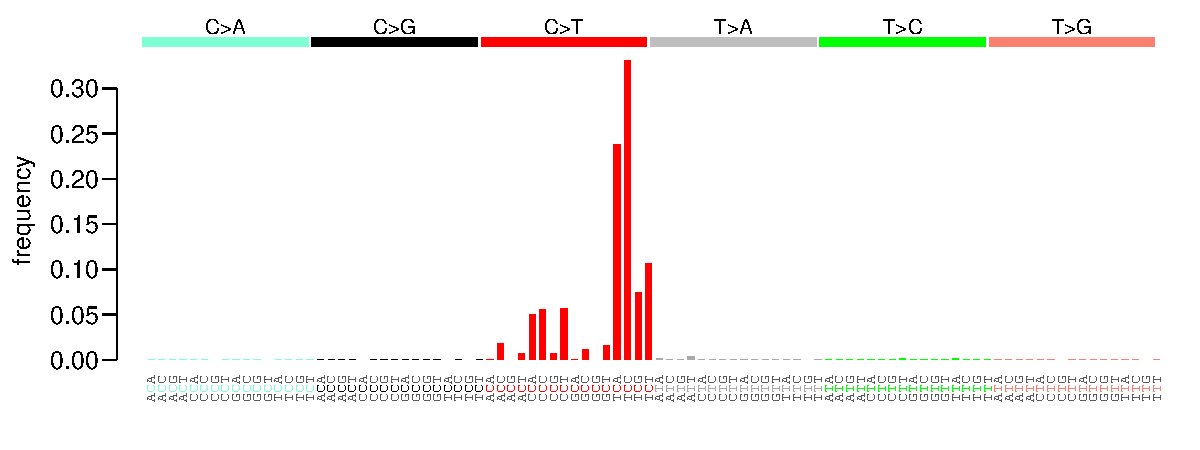
\includegraphics[width=.99\linewidth]{Figures/MisMatchFinder/SBS7aSignature.pdf}
\caption[Trinculeotide count contributions for single base substitution (SBS) signature 7a]{Trinculeotide count contributions for SBS signature 7a (UV exposure); values taken from \protect\textcite{Alexandrov2020}}\label{fig:sig7a}
\end{figure}

Additionally to the single base substitution (SBS), there exists doublet base substitution signatures (DBS) and InDel signatures for somatic mutations of cancers \cite{Alexandrov2020}, which are all based on the same principle and enable a higher precision for stratification of similar cancer subtypes and DNA damaging agents.

\subsection{Restrictions and pitfalls of standard signature analysis}
Especially for cancer samples, the focus, when analysing mutational signatures, is on somatic variants of the sample. \change{This}{Somatic variant calling, however,} requires deep sequencing of the tumour sample with at least WES or WGS. For optimal results, a  matched germline sample for tumour-normal variant calling is required (\autoref{intro-sec:somaticcalling}). This means the \change{cost of the assay}{assay cost} is surprisingly high for the diffuse result of signature contributions of the variants in the sample. This \add{cost overhead }is especially relevant when it comes to clinical diagnostic tools, where every biopsy of the patient is precious and not easily obtained. Additionally, the matched germline sample might not be available. For an analysis\remove{, which is} based on the averaged and aggregated somatic variants\change{, to require a}{ requiring} high-quality input \change{could be seen as}{is} counter-intuitive. \change{Especially}{Particularly} as the current gold standard analysis will report signatures, even if \change{there are virtually no variants}{virtually no variants are} reported\change{. W}{, w}e \remove{therefore }developed a method \change{which}{that} can be adapted for low coverage whole genome sequencing and requires no prior knowledge of the cancer or \change{a}{the} germline sample. \add{With this new method, we were able to analyse sequencing data, where normal variant calling is not possible due to the low and sparse read coverage.}

\subsection{Overview}
This chapter describes a newly developed method\change{, which}{ that} allowed the detection of somatic signatures from low-coverage WGS of cfDNA. \change{This method, w}{W}ith further optimisation and validation, \change{has the potential to}{this method can} provide a novel approach for non-invasive monitoring of patients and  screening of at-risk individuals in a clinical setting.
